\chapter{Monocular Scale}

\section{Introduction}

Recovering camera 6-DOF ego-motion from images is a well studied
problem. It arises in various practical contexts
(e.g. virtual/augmented reality application, autonomous or aided
navigation, etc.).  The problem was studied in both stereo and the
monocular setups.  To recover the full 6-DOF motion, the previous
works resorted to the stereo setup, used auxiliary sensors (e.g. IMU)
or made assumptions about the camera pose and the scene.  All of these
have their drawbacks: stereo pairs are fragile and require careful
calibration procedures, additional sensors are not always available
and also require calibration, scene assumptions don't always hold.
Motion estimation from images of a single moving camera is probably
the hardest setup, as well as the most desirable one, because of its
simplicity.  It is well known that the translation scale parameter is
not directly observable for a motion of a single camera.

We argue, that for natural scenes the scale information is present in
the images and may be extracted.  Our method learns a regressor, that
is capable to prediction the motion scale.

\section{Related work}
\paragraph{Geometry based methods} One category of works proceed by
making assumptions on the camera motion,
e.g.,~\cite{scaramuzza2009absolute}.  The authors assume that the
vehicle adheres to the Ackerman steering principle and exploit the
non-holomicity of the vehicle motion, to compute the exact scale of
the camera motion.  Other works make assumptions about the scene
(e.g., a presence of the planar surface in front of the vehicle) and
the height of the camera, e.g.~\cite{zhou2016reliable}, where the
authors estimate the ground plane homography that relates subsequent
images.  The motion scale is estimated/refined based on the homography
that relates the ground plane in subsequent images.
\paragraph{Learning methods} We are not aware of works that learn the
scale, rather there are a number of methods that use machine learning
approaches to tackle the visual odometry.  One such work
is~\cite{wang2017deepvo} that trains LSTM to predict the full 6-DOF
motion of the camera over sequences of
images. In~\cite{muller20017flowdometry} the authors use optical flow
images as CNN input to learn and infer camera motion. Authors
in~\cite{DBLP:journals/corr/MohantyADGSC16} also propose to train a
CNN.



\subsection{Our method}

We assume that a single camera moves through space and takes images.
We treat the initial camera pose (at time $t=0$) as the world
coordinate frame.  We denote the pose of the camera at time $t$ by
$\mathbf{\hat{T}}_t$ described by the rotation matrix
$\mathbf{\hat{R}}_t$ and the translation vector $\mathbf{\hat{t}}_t$
as seen in the world coordinate frame.  We denote camera image taken
at time $t$ by $I_t$.  To facilitate the discussion, we also introduce
notation for camera pose
$\mathbf{T}_t = [\mathbf{R}_t\ |\ \mathbf{t}_t] $ as seen from the
coordinate frame associated with camera pose at time $t-1$.  Most of
the time, we will omit the time index, since its clear from the
context.  By translation scale (or simply, scale) we refer to the norm
of the translation vector $\mathbf{t}$ (e.g.,
$s = \lVert \mathbf{t} \rVert$)

We pose the scale estimation problem as a regression problem and
search for a good regressor model.

\section{Random forest}

\subsection{Decision trees}

In this section we briefly describe tree-based methods for regression.
These involve splitting the feature space into a number of small
regions.  The prediction for a sample is made by computing a mean or a
mode of training samples that belong to the same region.  Since the
set of rules used to split the feature space into smaller regions may
be described by a tree, these methods are referred to as
\textit{decision tree} methods.

Building a decision tree may be described by a two step procedure:
\begin{enumerate}
\item Split the feature space, e.g., the set of all possible values
  for $X_1, X_2,\ldots,X_n$ into $J$ distinct regions $R_1, R_2,\ldots, R_J$.
\item For every sample that belongs to the regions $R_i$ we make the
  same prediction, which is a mean of the responses of training
  samples that belong to this region.
\end{enumerate}

The regions $R_i$ are usually chosen to be multidimensional boxes (axis aligned).  We would like to find such a partition of the feature space that minimizes
\begin{equation}\label{eq:tree_objective}
\sum\limits_{j=1}^J\sum_{x\in R_j}{(x-\mean{x}_j)^2}
\end{equation}

Where $\mean{x}_j$ denotes the mean of the response values of the
samples in region $R_j$.  Unfortunately, solving the optimization
problem~\ref{eq:tree_objective} is computationally hard.  Usually it
is replaced with a greedy algorithm, called \textit{recursive binary
  splitting}.  This approach starts at the top of the tree and
greedily chooses the best split at that point that minimizes the
variance of its sub-trees.  To be more precise, for each $j$ and $s$ we
define the hyper-planes:

\begin{equation}
  R_1(j,s) = \{ X\lvert X_j<s \}\quad\text{and}\quad R_2(j,s) = \{ X\lvert X_j \geq s \},
\end{equation}

We seek such $j$ and $s$ that minimize the equation:

\begin{equation}
  \sum\limits_{i:x_i\in R_1(j,s)}{(y_i-\hat{y}_{R_1})}^2 + \sum\limits_{i:x_i\in R_2(j,s)}{(y_i-\hat{y}_{R_2})}^2,
\end{equation}

Where $y_{R_1}, y_{R_2}$ are the average responses of the samples in
$R_1(j,s), R_2(j,s)$ respectively.  Once we found the $j$ and $s$ we
recursively split each sub-tree in a similar manner.  The process is
repeated until a stopping criterion (e.g., number of nodes in the
leaf) is reached.

\subsection{Bagging}
Decision trees tend to suffer from \textit{high variance}. This means
that if we split the training set into a number of random subsets and
fit random tree into each sub-sample, we would likely to get much
different answers from these trees when asked the same question.  It
is known that the variance of a mean of a set of independent random
variables is $\frac{1}{n}$.  Thus, in order to improve the variance of
the estimator, it is possible to fit $n$ estimators, each to its
training-set and the average their predictions.  Since, usually, we
don't have $n$ training sets, we would use \textit{bootstrapping}
(e.g., sample independently with replacement from the data set).

\subsection{Random Forest}
The random forest suggests an additional improvement over bagging, by
decorrelating the random trees.  The issue they attempt to address is
this: lets say there is a very dominant feature w.r.t. to task at hand
for a given data-set.  Bagging ensures that we use different training
sets, but yet, most trees will tend to first split on this dominant
feature.  In this case the trees will resemble each other.  In random
forest, the trees are constructed by using only a subset of features
(e.g., $m = \sqrt{p}$).  This means that at calculating the splits,
the algorithm is allowed to consider only a subset of features.

\section{Convolutional Neural Networks}

Convolutional neural networks (CNN) leverage the availability of the
computational power and the abundance of data.  CNN have become a
method of choice in a number of computer vision areas (e.g., image
classification~\cite{krizhevsky2012imagenet} ~\cite{simonyan2014very},
~\cite{szegedy2015going}, object recognition
~\cite{sermanet2013overfeat}~\cite{girshick2014rich}
~\cite{he2014spatial}.  They were also shown capable of per-pixel
tasks, such as semantic segmentation
~\cite{ning2005toward}~\cite{gupta2014learning}, depth estimation from
a single image ~\cite{liu2016learning}, optical flow
estimation~\cite{fischer2015flownet}.

Network architecture is a choice that needs to be made a priori.  To
best of our knowledge, there is no clear guideline on how to choose a
network architecture for a new task.  We experiment with two network architectures:

\begin{itemize}
\item the ZF~\cite{DBLP:journals/corr/ZeilerF13} object recognition
  network.  This is a more traditional CNN architecture.
\item the FlowNet~\cite{fischer2015flownet} optical flow estimation
  network.  This architecture adheres to a newer fully-convolutional
  family of networks.  These are known to train better and have less
  parameters vs. their fully-connected counterpart networks.
\end{itemize}

The input to our network is a pair of subsequent images.  A decision
to make is how to input the images into the network.  There are two
common choices: either create two siamese branches, so that each gets
its own input image, or to create a single multi-channel image.
~\cite{fischer2015flownet} show that the latter works equally well
while being simpler, so we choose to concatenate the images along the
channel dimension to produce a single 6-channel (for color) or
2-channel (for gray-scale) image.

\subsection{ZF}

The network architecture consists of five convolutional and three fully connected layers.  Table~\ref{tab:zf_geometry} summarizes the architecture.

\begin{table}[ht]
  \begin{tabular}{lcccc}
    \toprule
    \textbf{Layer} & \textbf{Receptive Field Size} & \textbf{Padding} & \textbf{Stride} & \textbf{Number of Channels}\\
    \midrule
    conv1&  $7\times 7$& 2& 3&   96\\
    conv2&  $5\times 5$& 2& 2&  256\\
    conv3&  $3\times 3$& 1& 1&  384\\
    conv4&  $3\times 3$& 1& 1&  384\\
    conv5&  $3\times 3$& 1& 1&  256\\
    fc6&               &  &  & 4096\\
    fc7&               &  &  & 4096\\
    fc8&               &  &  &    1\\
  \end{tabular}
  \caption{ZF network geometry}
  \label{tab:zf_geometry}
\end{table}

The flow of data through the network
\begin{figure}
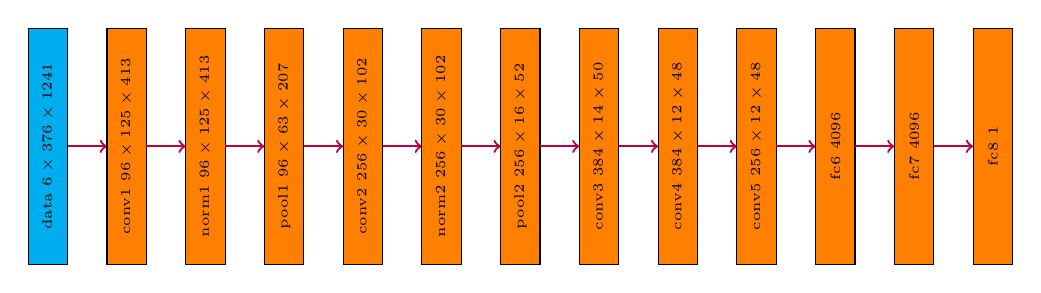
\begin{tikzpicture}
\draw[fill=cyan] (1.0, 0) rectangle (1.5, 3.0);
\draw[->, thick, purple] (1.5, 1.5) --(2.0, 1.5);
\node[font=\tiny, rotate=90] at (1.25, 1.5) {data $6\times 376\times 1241$};
\draw[fill=orange] (2.0, 0) rectangle (2.5, 3.0);
\draw[->, thick, purple] (2.5, 1.5) --(3.0, 1.5);
\node[font=\tiny, rotate=90] at (2.25, 1.5) {conv1 $96\times 125\times 413$};
\draw[fill=orange] (3.0, 0) rectangle (3.5, 3.0);
\draw[->, thick, purple] (3.5, 1.5) --(4.0, 1.5);
\node[font=\tiny, rotate=90] at (3.25, 1.5) {norm1 $96\times 125\times 413$};
\draw[fill=orange] (4.0, 0) rectangle (4.5, 3.0);
\draw[->, thick, purple] (4.5, 1.5) --(5.0, 1.5);
\node[font=\tiny, rotate=90] at (4.25, 1.5) {pool1 $96\times 63\times 207$};
\draw[fill=orange] (5.0, 0) rectangle (5.5, 3.0);
\draw[->, thick, purple] (5.5, 1.5) --(6.0, 1.5);
\node[font=\tiny, rotate=90] at (5.25, 1.5) {conv2 $256\times 30\times 102$};
\draw[fill=orange] (6.0, 0) rectangle (6.5, 3.0);
\draw[->, thick, purple] (6.5, 1.5) --(7.0, 1.5);
\node[font=\tiny, rotate=90] at (6.25, 1.5) {norm2 $256\times 30\times 102$};
\draw[fill=orange] (7.0, 0) rectangle (7.5, 3.0);
\draw[->, thick, purple] (7.5, 1.5) --(8.0, 1.5);
\node[font=\tiny, rotate=90] at (7.25, 1.5) {pool2 $256\times 16\times 52$};
\draw[fill=orange] (8.0, 0) rectangle (8.5, 3.0);
\draw[->, thick, purple] (8.5, 1.5) --(9.0, 1.5);
\node[font=\tiny, rotate=90] at (8.25, 1.5) {conv3 $384\times 14\times 50$};
\draw[fill=orange] (9.0, 0) rectangle (9.5, 3.0);
\draw[->, thick, purple] (9.5, 1.5) --(10.0, 1.5);
\node[font=\tiny, rotate=90] at (9.25, 1.5) {conv4 $384\times 12\times 48$};
\draw[fill=orange] (10.0, 0) rectangle (10.5, 3.0);
\draw[->, thick, purple] (10.5, 1.5) --(11.0, 1.5);
\node[font=\tiny, rotate=90] at (10.25, 1.5) {conv5 $256\times 12\times 48$};
\draw[fill=orange] (11.0, 0) rectangle (11.5, 3.0);
\draw[->, thick, purple] (11.5, 1.5) --(12.0, 1.5);
\node[font=\tiny, rotate=90] at (11.25, 1.5) {fc6 $4096$};
\draw[fill=orange] (12.0, 0) rectangle (12.5, 3.0);
\draw[->, thick, purple] (12.5, 1.5) --(13.0, 1.5);
\node[font=\tiny, rotate=90] at (12.25, 1.5) {fc7 $4096$};
\draw[fill=orange] (13.0, 0) rectangle (13.5, 3.0);
\node[font=\tiny, rotate=90] at (13.25, 1.5) {fc8 $1$};
\end{tikzpicture}
\caption{ZF network data flow.  Each rectangle depicts a top blob for a corresponding layer.}
\end{figure}

There is a last fully connected layer that reduces a network to a
single output, which we are interested to learn.  We use euclidean
loss to train the network.  Total number of parameters is about 624
million.


\subsection{FlowNet}

Fully-convolutional network is a recent trend in the field.  They are
known to train better and have less parameters vs. their fully
connected counterparts~\cite{long2015fully}. The geometry of the
network is described in Table~\ref{tab:flownet_geometry}. Each
convolutional layer is followed by the non-linearity.  We chose this
architecture since it proved successful for optical flow estimation
task and has pre-trained model readily available.

\begin{table}[ht]
  \begin{tabular}{lcccc}
    \toprule
    \textbf{Layer} & \textbf{Receptive Field Size} & \textbf{Padding} & \textbf{Stride} & \textbf{Number of Channels}\\
    \midrule
    conv1&   $7\times 7$& 3& 2&   64\\
    conv2&   $5\times 5$& 2& 2&  128\\
    conv3&   $5\times 5$& 2& 2&  256\\
    conv3-1& $3\times 3$& 1& 1&  256\\
    conv4&   $3\times 3$& 1& 2&  512\\
    conv4-1& $3\times 3$& 1& 1&  512\\
    conv5&   $3\times 3$& 1& 2&  512\\
    conv5-1& $3\times 3$& 1& 1&  512\\
    conv6&   $3\times 3$& 1& 2& 1024\\
    conv6-1& $3\times 3$& 1& 1& 1024\\
    conv7&   $3\times 3$& 1& 2&    1\\
    \hline
  \end{tabular}
  \caption{Geometry of the FlowNet based network}
  \label{tab:flownet_geometry}
\end{table}

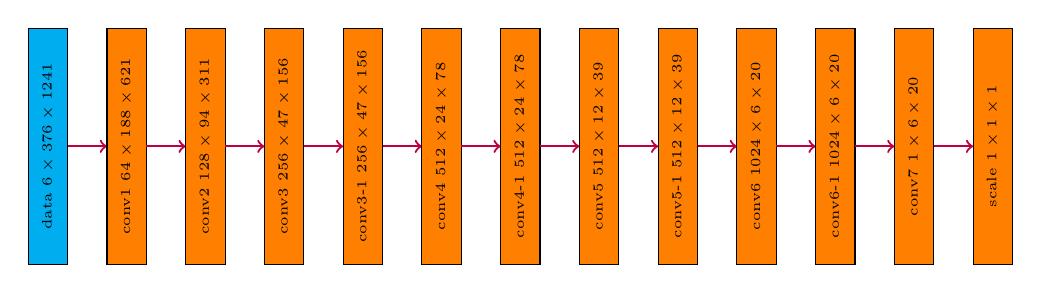
\begin{tikzpicture}
\draw[fill=cyan] (1.0, 0) rectangle (1.5, 3.0);
\draw[->, thick, purple] (1.5, 1.5) --(2.0, 1.5);
\node[font=\tiny, rotate=90] at (1.25, 1.5) {data $6\times 376\times 1241$};
\draw[fill=orange] (2.0, 0) rectangle (2.5, 3.0);
\draw[->, thick, purple] (2.5, 1.5) --(3.0, 1.5);
\node[font=\tiny, rotate=90] at (2.25, 1.5) {conv1 $64\times 188\times 621$};
\draw[fill=orange] (3.0, 0) rectangle (3.5, 3.0);
\draw[->, thick, purple] (3.5, 1.5) --(4.0, 1.5);
\node[font=\tiny, rotate=90] at (3.25, 1.5) {conv2 $128\times 94\times 311$};
\draw[fill=orange] (4.0, 0) rectangle (4.5, 3.0);
\draw[->, thick, purple] (4.5, 1.5) --(5.0, 1.5);
\node[font=\tiny, rotate=90] at (4.25, 1.5) {conv3 $256\times 47\times 156$};
\draw[fill=orange] (5.0, 0) rectangle (5.5, 3.0);
\draw[->, thick, purple] (5.5, 1.5) --(6.0, 1.5);
\node[font=\tiny, rotate=90] at (5.25, 1.5) {conv3-1 $256\times 47\times 156$};
\draw[fill=orange] (6.0, 0) rectangle (6.5, 3.0);
\draw[->, thick, purple] (6.5, 1.5) --(7.0, 1.5);
\node[font=\tiny, rotate=90] at (6.25, 1.5) {conv4 $512\times 24\times 78$};
\draw[fill=orange] (7.0, 0) rectangle (7.5, 3.0);
\draw[->, thick, purple] (7.5, 1.5) --(8.0, 1.5);
\node[font=\tiny, rotate=90] at (7.25, 1.5) {conv4-1 $512\times 24\times 78$};
\draw[fill=orange] (8.0, 0) rectangle (8.5, 3.0);
\draw[->, thick, purple] (8.5, 1.5) --(9.0, 1.5);
\node[font=\tiny, rotate=90] at (8.25, 1.5) {conv5 $512\times 12\times 39$};
\draw[fill=orange] (9.0, 0) rectangle (9.5, 3.0);
\draw[->, thick, purple] (9.5, 1.5) --(10.0, 1.5);
\node[font=\tiny, rotate=90] at (9.25, 1.5) {conv5-1 $512\times 12\times 39$};
\draw[fill=orange] (10.0, 0) rectangle (10.5, 3.0);
\draw[->, thick, purple] (10.5, 1.5) --(11.0, 1.5);
\node[font=\tiny, rotate=90] at (10.25, 1.5) {conv6 $1024\times 6\times 20$};
\draw[fill=orange] (11.0, 0) rectangle (11.5, 3.0);
\draw[->, thick, purple] (11.5, 1.5) --(12.0, 1.5);
\node[font=\tiny, rotate=90] at (11.25, 1.5) {conv6-1 $1024\times 6\times 20$};
\draw[fill=orange] (12.0, 0) rectangle (12.5, 3.0);
\draw[->, thick, purple] (12.5, 1.5) --(13.0, 1.5);
\node[font=\tiny, rotate=90] at (12.25, 1.5) {conv7 $1\times 6\times 20$};
\draw[fill=orange] (13.0, 0) rectangle (13.5, 3.0);
\node[font=\tiny, rotate=90] at (13.25, 1.5) {scale $1\times 1\times 1$};
\end{tikzpicture}

We use Euclidean loss to train the network. The total number of
parameters is 24 million.

\section{Recurrent Neural Networks}

Many problems require passing information through time.  Since the
traditional neural networks are stateless, they are poorly suited for
this purpose. Recurrent Neural Networks have loops in them, so that
the information can persist.

\begin{figure}[h!]
  \centering 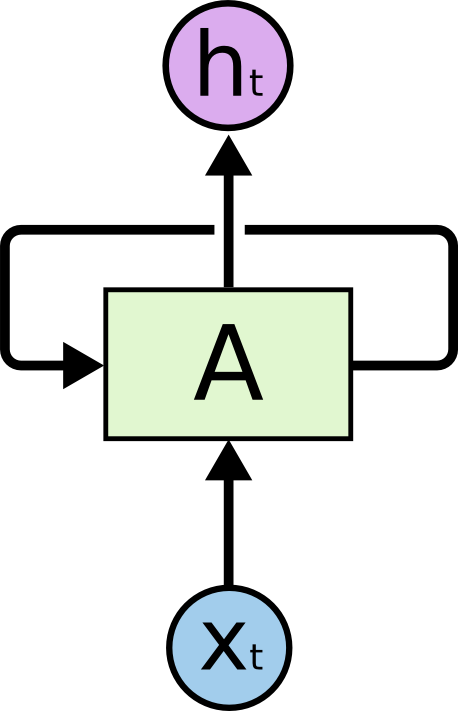
\includegraphics[width=0.15\textwidth]{RNN-rolled}
  \caption{RNN}
  \label{fig:rnn1}  
\end{figure}

In the Figure~\ref{fig:rnn1} network $A$ accepts input $x_t$ and
outputs $h_t$.  The loop allows the network to pass information from
one step of to another.

The RNN may be thought of as a chain of multiple copies of the same
neural network where each node passes a message to its successor.
This is called \textit{network unrolling}, depicted in
Figure~\ref{fig:rnn2}.  Unrolled network stresses the relation of the
RNN to the sequential data streams.  This is an architecture of choice
when modeling such data.

\begin{figure}[ht!]
  \centering 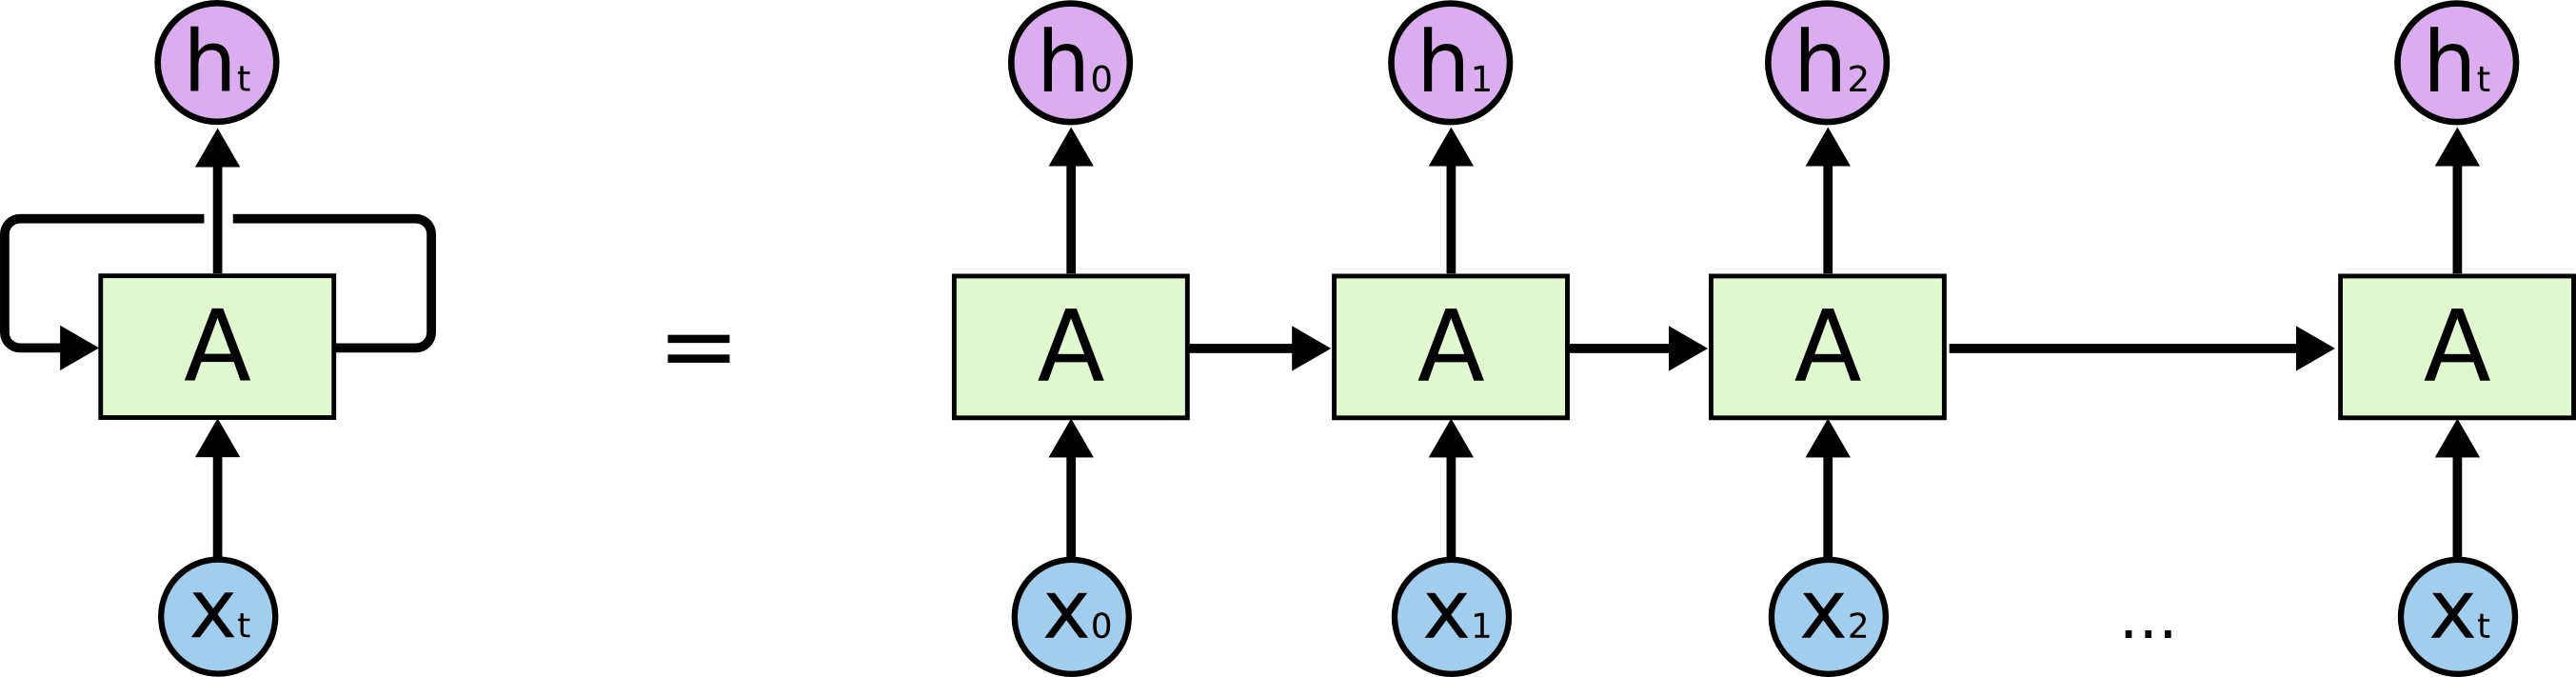
\includegraphics[width=.7\textwidth]{RNN-unrolled}
  \caption{An unrolled RNN}\label{fig:rnn2}
\end{figure}

It turns out that the vanilla RNN are hard to train due to the
exploding/imploding gradients.  Fortunately, Long Short Term Memory
Networks (LSTM), which is a special kind of RNN addresses these issues.

LSTM were introduced by~\cite{hochreiter1997long}, they are
specifically designed to model long term dependencies. Similarly to
RNN, LSTM posses a chain-like structure. Each repeating node has an
internal structure depicted in Figure~\ref{fig:lstm1}.

\begin{figure}[ht!]
  \centering 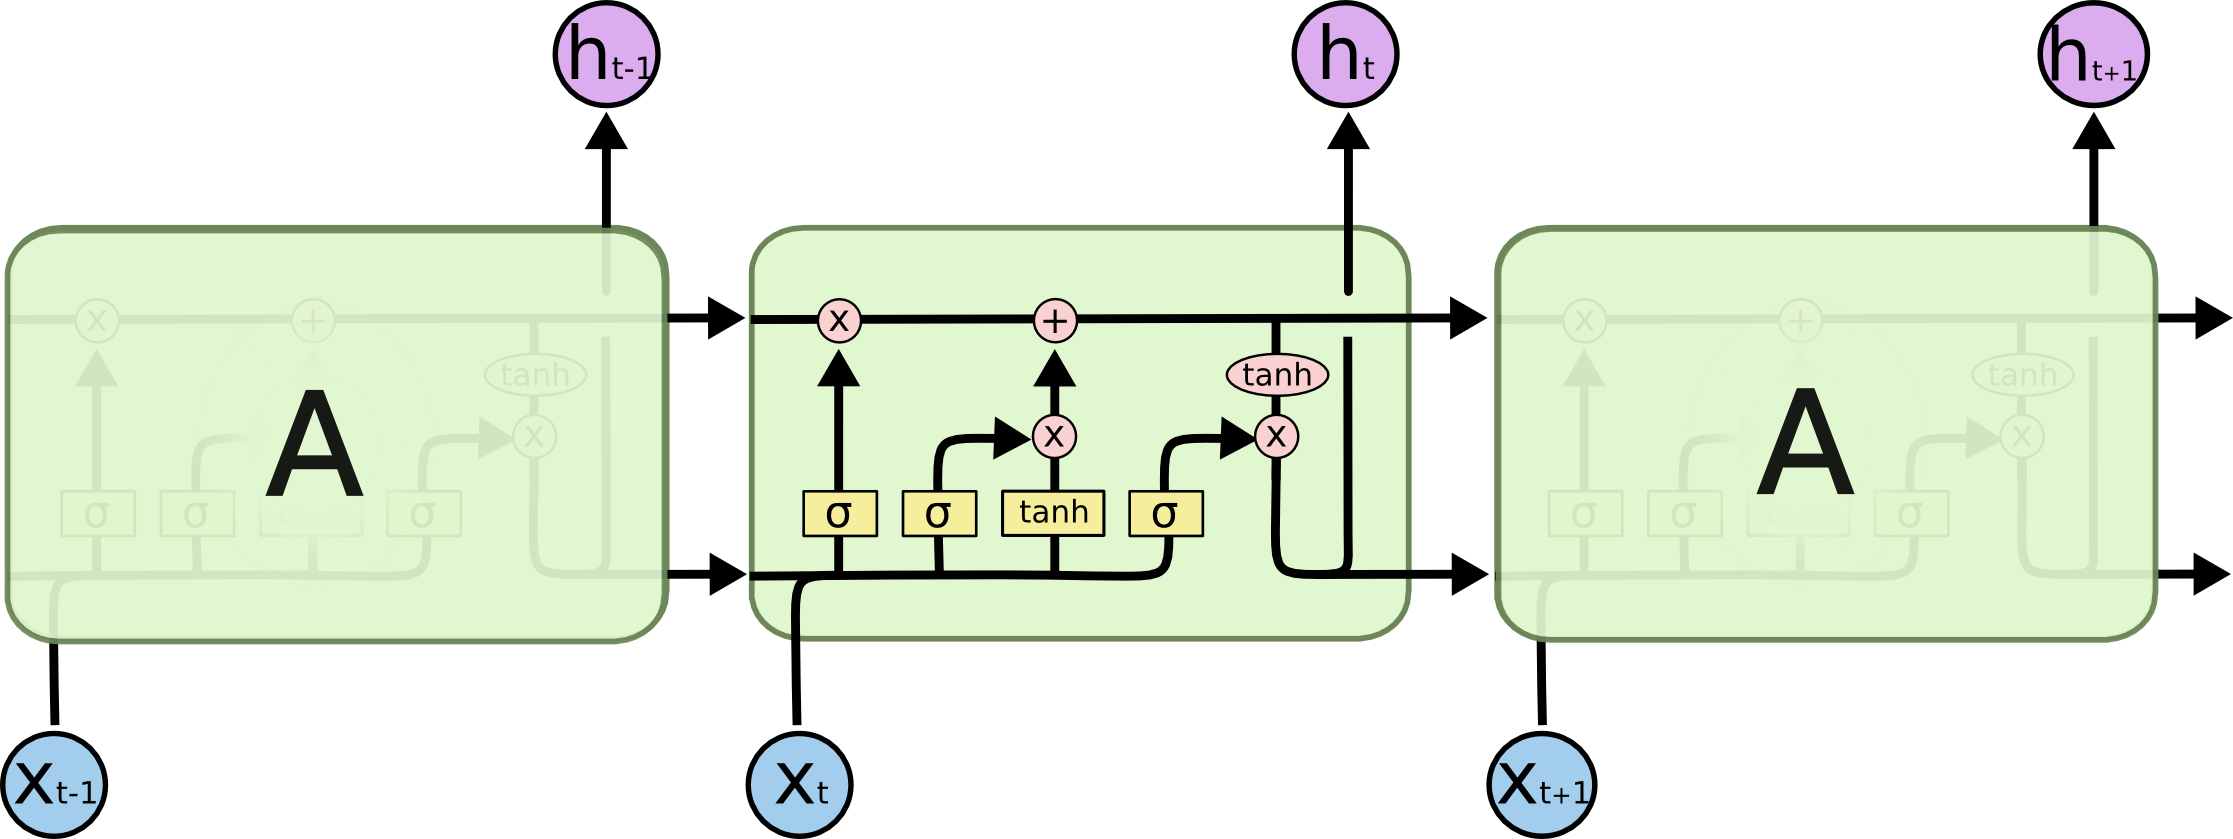
\includegraphics[width=.7\textwidth]{LSTM3-chain}
  \caption{Long Short Term Memory}\label{fig:lstm1}
\end{figure}

\begin{figure}[ht!]
  \centering 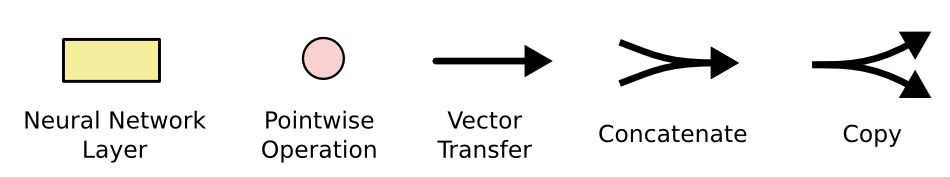
\includegraphics[width=.5\textwidth]{LSTM2-notation}
  \caption{A notation used in Figure~\ref{fig:lstm1}}\label{fig:lstm2}
\end{figure}

To use the LSTM for the image data we combine the convolutional
network with the LSTM.  $X_t$ vectors are produced by the ZF convnet.
This is a fairly common representation used previously.  The convnet
and the LSTM are trained jointly.

The geometry of the network is as follows:
\begin{itemize}
\item conv1: (96, 6, 7, 7)
\item conv2: (384, 48, 5, 5)
\item conv3: (512, 384, 3, 3)
\item conv4: (512, 256, 3, 3)
\item conv5: (384, 256, 3, 3)
\item fc6:   (4096, 34560)
\item lstm1: (1024, 4096)
\item fc-final: (1, 256)
\end{itemize}
Total number of trainable parameters is about 150 millions.

\section{Experiments}

\subsection{Data-set}

We train and test on the KITTI data-set~\cite{geiger2013vision}.  The
data-set consists of 11 sequences with ground truth data.  We
arbitrarily use sequence 00 for testing and sequences 01-10 for
training.  There are 4540 and 18650 images in the test and the train
sets respectively. We only use the data from the left color camera.
Figure~\ref{fig:scales} depicts the distribution of the scale values
over the train and the test sets.

\begin{figure}[!ht]
  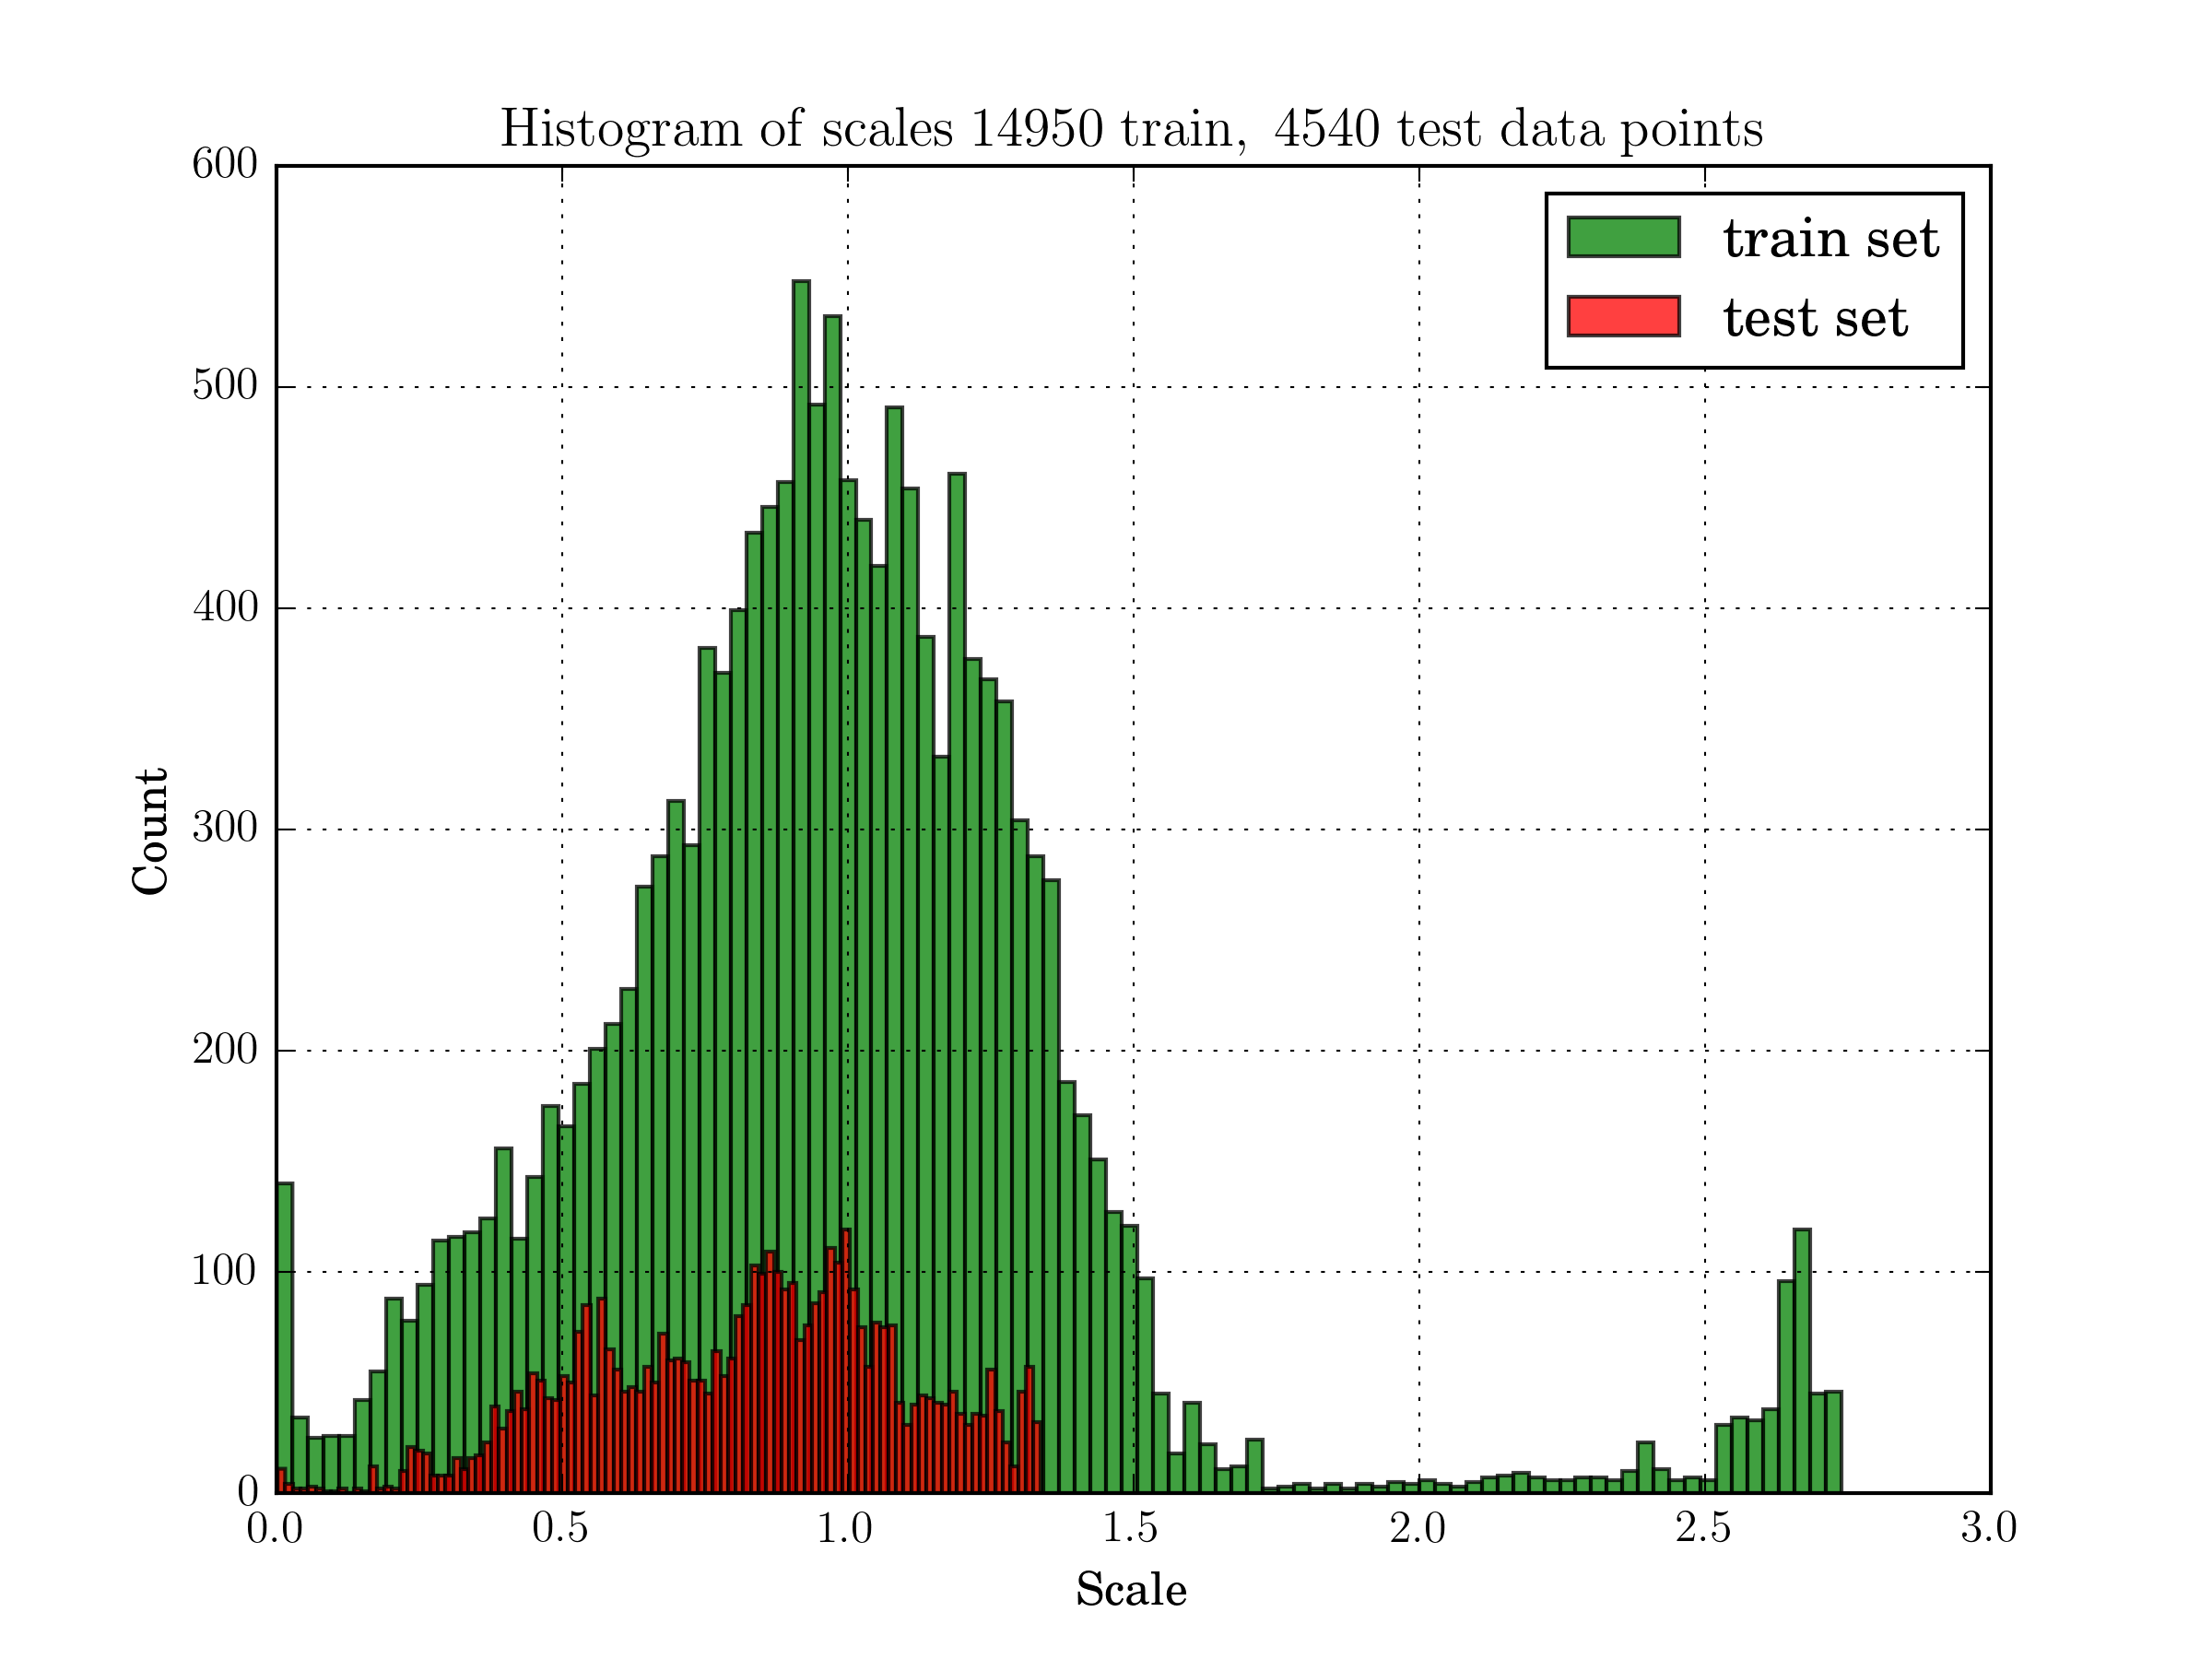
\includegraphics[width=0.9\linewidth]{no_00-scales}
  \caption{The train set}
  \label{fig:stats-no_00}
  \caption{Scale distributions}
  \label{fig:scales}
\end{figure}

\subsection{Random Forest}

\subsection{Feature Extraction}\label{sec:features}

In order to train the random forest we need to represent subsequent
image pairs as feature vectors, which are created as follows: we
extract and match sparse salient points in both input images.  The
output of this stage is a set of a corresponding pixel locations.
Then, we compute the point displacement magnitudes.  Finally, we bin
all the interest pundits according to a grid and create histogram of
displacement magnitudes for each bin.  Concatenating all histograms
together produces a feature vector. We use Harris corners and square
$11\times 11$ patches as corner descriptors. Sum of square differences
is used as a distance measure with the winning pair declared a match.
To prune the outliers we fit the fundamental matrix into the matched
corner sets and remove the corners that do not agree with the model.
Figure~\ref{fig:ex_corner_and_matching} shows a typical example of
extracted and matched corners.


Some statistics of the features is presented in the
Figure~\ref{fig:feature_vectors}. We expect the peaks, that correspond
to a closer image regions have a distributions shifted to the right
(i.e., larger displacements) and the peaks that correspond to a
regions farther away should be closer to zero.  This behavior can be
observed especially well for the feature vectors that correspond to
larger camera displacements (e.g. Figure~\ref{fig:1c}).

\begin{figure}[!ht]
  \centering
  \begin{subfigure}{.45\linewidth}
    \centering
    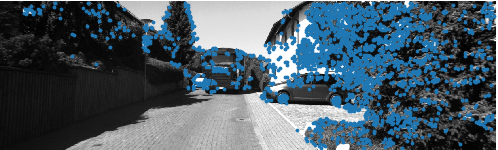
\includegraphics[width=\linewidth]{10_001157_001158_raw_corners_left}
    \caption{}
    \label{fig:ex_corner_and_matching:corner}
  \end{subfigure}
  \begin{subfigure}{.45\linewidth}
    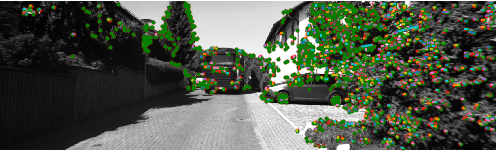
\includegraphics[width=\linewidth]{10_001157_001158_final_matches1}
    \caption{}
    \label{fig:ex_corner_and_matching:match}    
  \end{subfigure}
  \caption{Typical corner extraction and
    matching. Figure~\subref{fig:ex_corner_and_matching:corner} shows the raw
    extracted corners, while Figure~\subref{fig:ex_corner_and_matching:match} shows
    pruned and matched corners.}
  \label{fig:ex_corner_and_matching}
\end{figure}

\begin{figure}[!ht]
  \centering
  \begin{subfigure}{.45\linewidth}
    \centering
    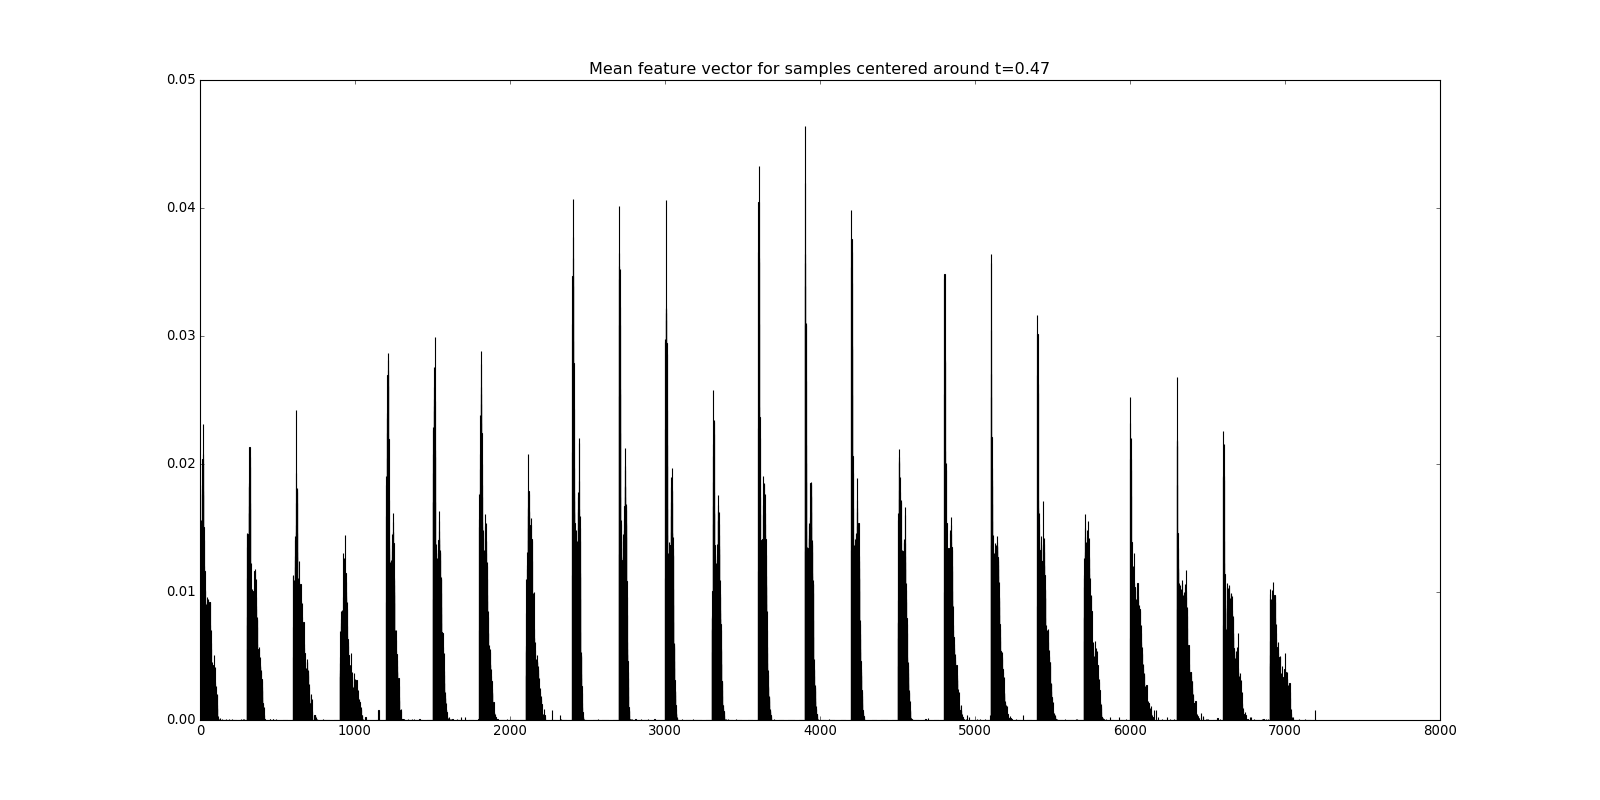
\includegraphics[width=1.2\linewidth]{00_mean_feature_vector_0_47}
    \caption{}\label{fig:1a}
  \end{subfigure}%
  \begin{subfigure}{.45\linewidth}
    \centering
    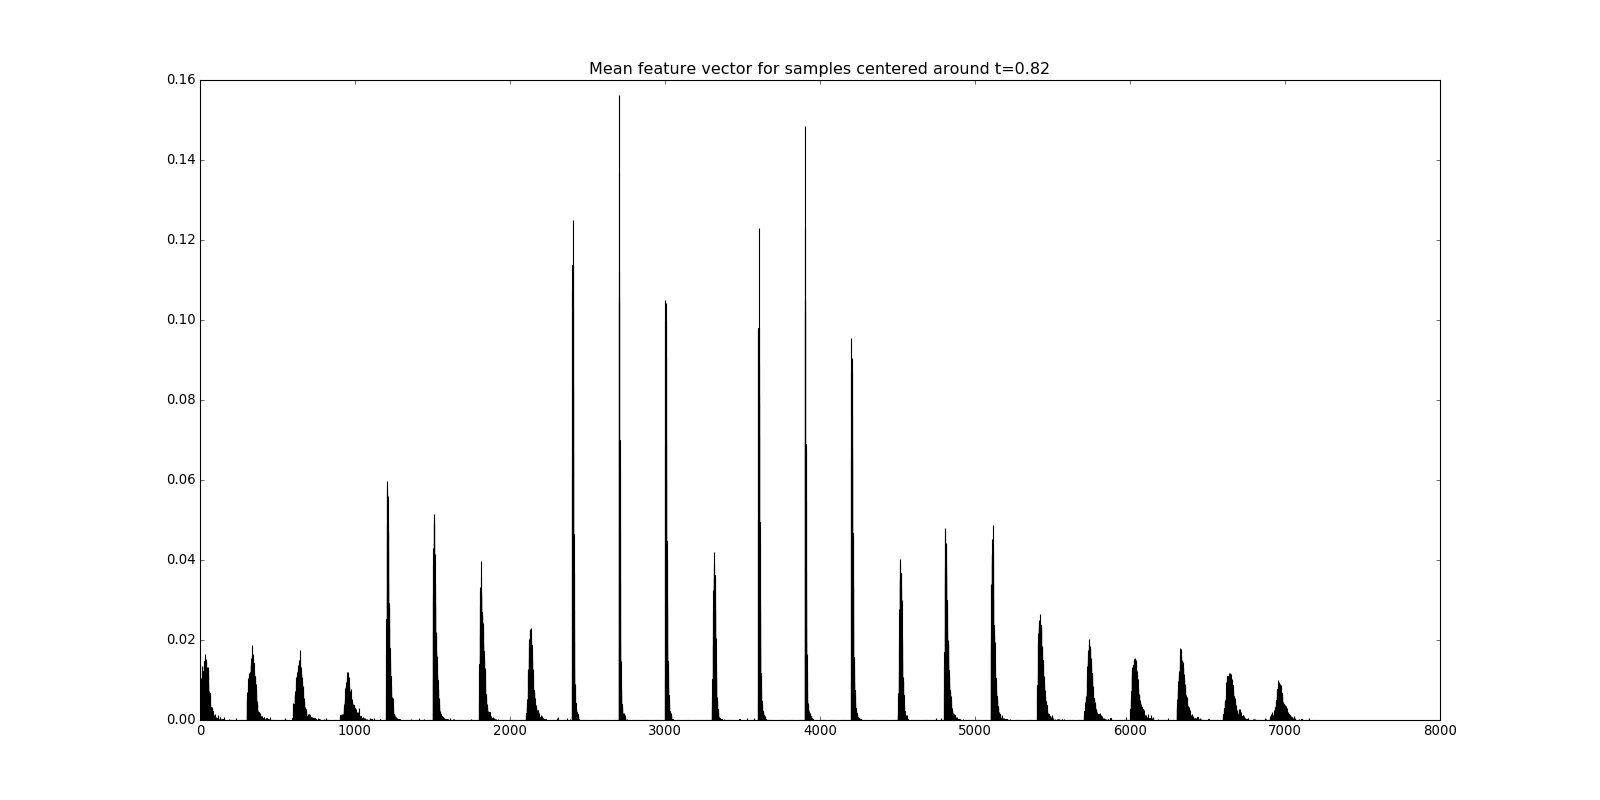
\includegraphics[width=1.2\linewidth]{00_mean_feature_vector_0_81}
    \caption{}\label{fig:1b}
  \end{subfigure}%
  \\
  \begin{subfigure}{\linewidth}
    \centering
    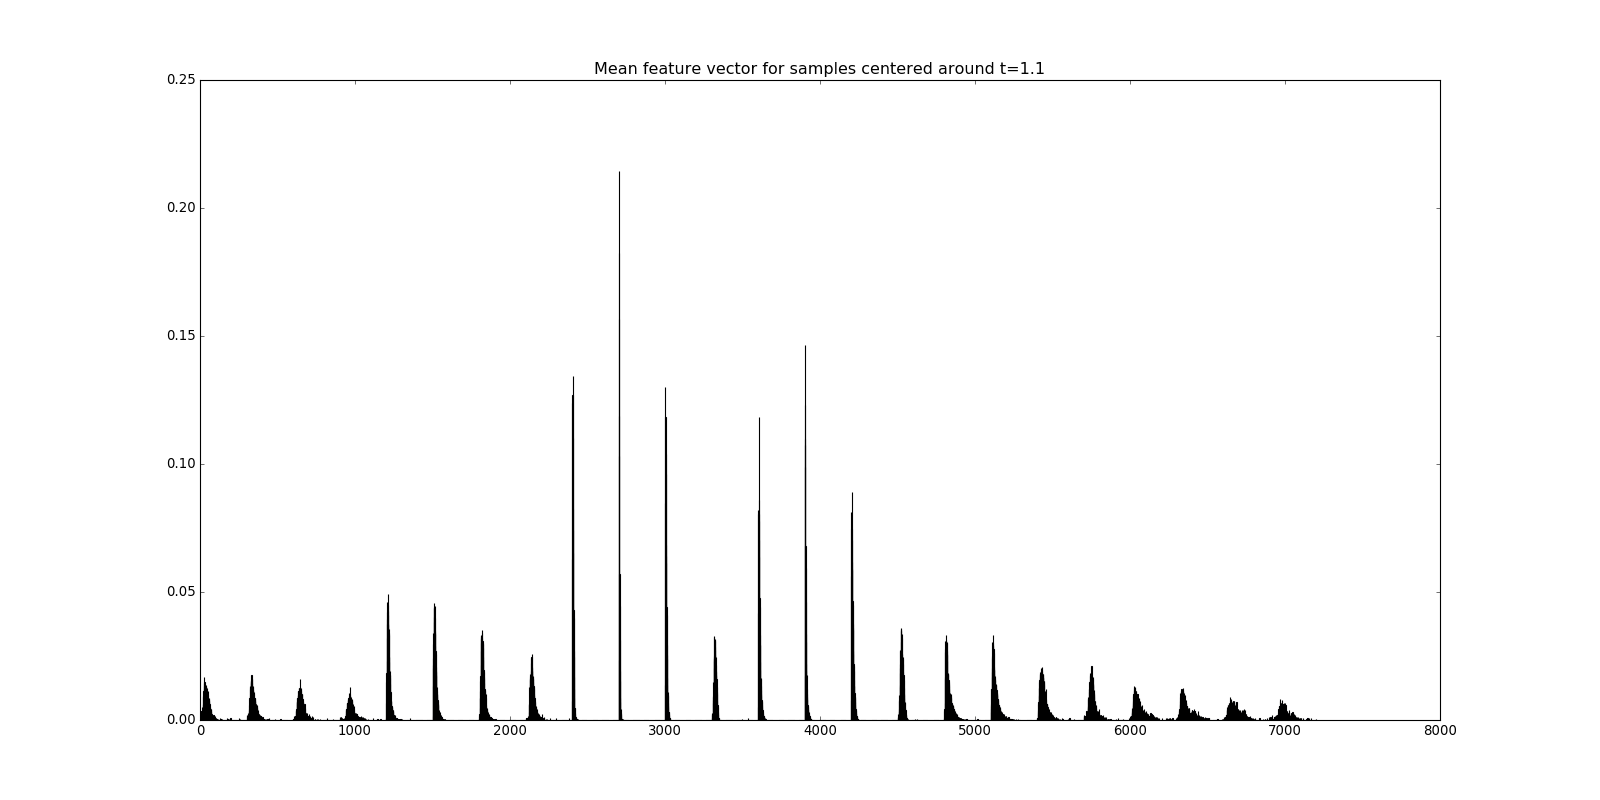
\includegraphics[width=.8\textwidth]{00_mean_feature_vector_1_1}
    \caption{}\label{fig:1c}
  \end{subfigure}%
  \caption{Average feature vectors for samples centered around the
    specific camera translation magnitude.  Each peak corresponds to a
    grid cell (e.g. here the grid is 4 rows by 6 columns by 300 bins,
    so the feature vector is of the dimension 6*4*300=7200).  The grid
    is sampled in a column-major mode. So the first four peaks
    correspond to the leftmost column of the image grid.}
  \label{fig:feature_vectors}
\end{figure}

We bin each image into $6\times 4$ grid.  For each bin in the image we
compute the histogram of corner disparities.  By disparity we denote
the displacement of the corner in the image.  We use $300$-bin
histogram for disparities (e.g, feature vector length is $7200$).

We use the extracted features to fit a random forest, by means of
recursive note splitting with sub-node variance minimization. The mean
absolute error is 0.174 meters with a standard deviation of 0.148
meters.

\section{Neural networks}

We use Caffe~\cite{jia2014caffe} framework to train and test our
models.
\paragraph{ZF} We train using vanilla SGD for 100 epochs and decrease
learning rate by factor of .1 every 10 epochs. We train the network
from scratch.
\paragraph{FlowNet} We also train using vanilla SGD for 100 epochs
decreasing learning rate by .1 every 10 epochs.  We start from
pre-trained weights of~\cite{fischer2015flownet}.
\paragraph{LSTM} TBD

\section{Results}

Let the ground truth sequence of camera motion scales by
$\{y_i\}_{i=0}^N$.  Let the predicted scales for the same sequence be
$\{\hat{y}_i\}_{i=0}^N$.  We report the mean absolute error:
\[
  \mu = \frac{1}{N}\sum_0^N{|y_i - \hat{y}_i|}
\]

\begin{table}[ht]
  \centering
  \begin{tabular}{ lcccc }
    \hline
                        & Random Forest & ZF   & FlowNet & LSTM ZF \\
    \hline
    $\mu\quad[meters]$        & .237          & .200 & \textbf{.103}    & .198 \\
    $\sigma\quad[meters]$     & .229          & .161 & \textbf{.08}     & .147 \\    
    \hline
  \end{tabular}
  \caption{Experimental Results}
  \label{table:1}
\end{table}


%%% Local Variables:
%%% mode: latex
%%% TeX-master: "../thesis"
%%% End:
